\newpage
\appendix

\section{Implementation details}
\label{sec:appendix_implementation}

  In this section, we provide details about the implementations of the baselines and our models. Appendix \ref{sec:appendix_results} provides details and additional results for each environment we used.

\subsection{LoP-PPO}
\label{subsec:lopppo}

We detail the losses used in algorithm \ref{alg:lop_ppo}. First, we recall the clipped-PPO surrogate objective described in \cite{ppo}. For a given trajectory $\tau=\left \{(s_t,a_t,r_t)\right \}_{0}^T$ collected by the policy $\pi_{\theta_{old}}$, and denoting $\rho_t\left ( \theta \right )=\frac{\pi_{\theta}(a_t|s_t)}{\pi_{\theta_{old}}}$, the goal is to maximize:
\begin{equation}
\widehat{\mathcal{L}}_{PPO} \left ( \theta \right ):=\frac{1}{T}\sum_{t=0}^{T}\min{\left [\rho_t\left ( \theta \right )A^{\pi_{\theta_{old}}}\left (s_t,a_t \right ), clip\left (\rho_t\left ( \theta \right ),1+\epsilon,1-\epsilon \right )A^{\pi_{\theta{old}}}\left (s_t,a_t \right ) \right ]}
\end{equation}

Where function $A^{\pi_{\theta_{old}}}$ is computed thanks to a value function $V_{\phi}$ by using Generalized Advantage Estimation (\cite{GAE}). This function is simultaneously updated by regression on mean-squared error over the rewards-to-go $\widehat{R}_t$. In our case, this function not only takes $s_t$ as an input, but also the value $z$:

\begin{equation}
\widehat{\mathcal{L}}_{MSE} \left ( \phi,z \right ):=\frac{1}{T}\sum_{t=0}^{T}\left ( V_{\phi}\left ( s_t,z \right )-\widehat{R}_t \right )^2
\end{equation}

In HalfCheetah and Ant experiments, we sampled actions from a reparametrized Gaussian distribution using a squashing function (\cite{squashing}), but we set the standard deviation fixed (so it is an hyper-parameter encouraging exploration, called \textit{action std} in Tables \ref{table:hp_halfcheetah} and \ref{table:hp_ant}): the policy network only learns the mean of this distribution. 

\subsection{BoP and CoP}
\label{subsec:bopcop}

The only change between LoP and these models resides in the way we combine the $N$ anchor policies. For CoP, it is just the generalization of LoP for $N>2$ (see \ref{sec:subspaces}).  BoP, makes use of a Bezier parametric curve that uses Bernstein polynomials (the anchor parameters being the \textit{control points}). For $N=3$, it is defined by:
\begin{equation}
\bar\Theta=\left \{(1-z)^2\:\bar\theta_1\:+\:2\left ( 1-z \right )z\:\bar\theta_2 \:\: + \: z^2\:\bar\theta_3,\:\:\: \forall z\in[0,1]\right\}
\end{equation}
 Concerning the policies $z$ evaluated at test time,  BoP uses the same strategy as LoP by testing values that are uniformly distributed in $[0;1]$. For CoP, we opted for sampling $K$ policies using a Dirichlet distribution over $[0,1]^3$.
 
\subsection{DIAYN+R and Lc}
\label{subsec:diayn_lc}
In order to find the best trade-off between maximizing environment rewards and intrinsic rewards in DIAYN+R algorithm, we add the hyper-parameter $\beta$ :
\begin{equation}
    R_{DIAYN+R}(s,a) = r(s,a) + \beta \cdot \log p(z|s)
\end{equation}

As an alternative to DIAYN+R \cite{Tokyo} proposes an algorithm where the discriminator takes not only observations as an input but also the policy output, updating both discriminator $q_\phi$ and policy $\pi_\theta$ when back propagating the gradient. In this case, it is not necessary to add an intrinsic reward. While \cite{Tokyo} illustrate their methods with TD3 and SAC, we adapted it to PPO. The surrogate loss is given by:

\begin{equation}
\mathcal{L}_{LC}:=\:\widehat{\mathcal{L}}_{PPO}\:+\:\beta\cdot\log q_{\phi}\left ( z \:|\:s,\pi_{\theta}\left ( .|s,z \right ) \right )
\end{equation}



% Where $\mu_\theta$ is the "raw" output of the policy network, and $W$ an importance weight over a batch of samples:
% \begin{equation}
% W = \frac{\exp\left ( Q\left ( s,a,z \right ) \right )}{\sum_{(\bar{s},\bar{a},\bar{z})\in\mathcal{D}_{batch}}\exp\left ( Q\left (\bar{s},\bar{a},\bar{z} \right ) \right )}
% \end{equation}

% In practice, this importance weight is clipped between $1-\epsilon$ and $1+\epsilon$, $\epsilon$ being a parameter to tune. In the off-policy variants, $\mathcal{D}_{batch}$ is sampled in a replay buffer. In our case, we simply performed a softmax over each minibatch and tested different values for $\epsilon$. 



% \subsection{Hyperparameters selection}
% \label{subsec:lcppo}
% For all the experiments, we proceeded as follows: we first performed a gridsearch on the vanilla algorithms (A2C and PPO), and then fixed the best hyperparameters for the other algorithms. Then we ran a smaller gridsearch on the specific hyperparameters of each algorithm. Here is the gridsearch performed for all experiments:
% \begin{itemize}
%      \item LoP: $\beta:\left \{0.1,1.,10. \right \}$
%      \item DIAYN+R: $\beta:\left \{0.1,1.,10. \right \}$,\:lr discriminator:$\left \{1e^{-4},1e^{-3} \right \}$
%      \item Lc: clipping weight: $\left \{0.3,0.2,0.1 \right \}$,\:lr discriminator:$\left \{1e^{-4},1e^{-3} \right \}$
%  \end{itemize}

%  To avoid any overfitting, the selections were made on the training environments and are reported on the subsections "hyperparameters" in \ref{sec:appendix_results}.

\newpage
\section{Experiments details and additional results}
\label{sec:appendix_results}


% \subsection{Details on baseline implementations}
% \label{subsec:baseline}


\subsection{HalfCheetah}
\label{subsec:halfcheetah}

Task originally coming from OpenAI Gym \citep{OpenaiGym}. Instead of using MuJoCo engine, we decided to use Brax \citep{brax2021github} as it enables the possibility to acquire episodes on GPU. We use the vanilla environment for training.The policy and the critic are encoded by two different multi-layer perceptrons with ReLU activations. The base learning algorithm is PPO.

\textbf{Test environments:} we operated modifications similar as the ones proposed in \citep{henderson2017multitask}. Morphological variations: we changed the radius and mass of specific body parts (torso, thig, shin, foot). Variations in physics: we changed the gravity and friction coefficients. \\
Table \ref{table:halfcheetah_test_setting} precisely indicates the nature of the changes for each environment.

\begin{table}[h!]
\centering
\begin{tabular}{l|l}
\textbf{Env name}&\textbf{Modifications} \\\midrule
BigFeet & Feet mass and radius $\times 1.25$ \\
BigFriction & Friction coefficient $\times 1.25$ \\
BigGravity& Gravity coefficient $\times 1.25$ \\
BigShins& Shins mass and radius $\times 1.25$ \\
BigThighs& Thighs mass and radius $\times 1.25$ \\
BigTorso& Torso mass and radius $\times 1.25$ \\
SmallFeet &Feet mass and radius $\times 0.75$ \\
SmallFriction &Friction coefficient $\times 0.75$ \\
SmallGravity&Gravity coefficient $\times 0.75$ \\
SmallShins &Shins mass and radius $\times 0.75$ \\
SmallThighs &Thighs mass and radius $\times 0.75$ \\
SmallTorso& Torso mass and radius $\times 0.75$ \\
HugeFriction & Friction coefficient $\times 1.5$ \\
HugeGravity &Gravity coefficient $\times 1.5$ \\
TinyFriction& Friction coefficient $\times 0.5$ \\
TinyGravity &Gravity coefficient $\times 0.5$ \\
\hline
\end{tabular}
\caption{Modified HalfCheetah environments used for testing. Morphological modifications include a variation on the mass and the radius of a specific part of the body (torso, thighs, shins, or feet). We also modified the dynamics (gravity and friction). Environment names are exhaustive: Big refers to a increase of 25\% of radius and mass, Small refers to a decrease of 25\%. For example, "BigFoot" refers to an HalfCheetah agent where feet have been increased in mass and radius by 25\%. For gravity and friction, we also tried an increase/decrease by 50\% (respectively tagged "Huge" and "Tiny").}
\label{table:halfcheetah_test_setting}
\end{table}

\newpage


\begin{table}[h!]
\begin{center}
\begin{tabular}{l|c} \toprule
   \textbf{Hyper-parameter} & \textbf{Value} \\ \hline
    lr policy: &  $0.0003$\\
    lr critic: &  $0.0003$\\
    n parallel environments: & $2048$ \\
    n acquisition steps per epoch: & $20$ \\
    batch size: & $512$ \\
    num minibatches: & $32$ \\
    update epochs: & $8$ \\
    discount factor: &  $0.99$\\
    clip ration: &  $0.3$\\
    action std: &  $0.5$\\
    gae coefficient: &  $0.96$\\
    reward scaling: &  $1.$\\
    gradient clipping: & $10.$ \\ 
    n layers (policy): & $4$ \\ 
    n neurons per layer (policy): & $64$ \\
    n layers (critic): & $5$ \\ 
    n neurons per layer (critic): & $256$ \\\toprule
    \multicolumn{2}{c}{LoP, BoP, CoP} \\ 
    \hline
    $\beta$: & $1$ \\\toprule
    \multicolumn{2}{c}{DIAYN} \\ 
    \hline
    $\beta$: & $0.1$ \\
    lr discriminator: &  $0.0001$\\
    n layers (discriminator): & $2$ \\ 
    n neurons per layer (discriminator): &  $64$\\\toprule
    \multicolumn{2}{c}{Lc} \\ 
    \hline
    $\beta$: & $10$ \\
    dimensions of z: &  $1$\\
    lr discriminator: &  $0.001$\\
    n layers (discriminator): & $2$ \\ 
    n neurons per layer (discriminator): &  $64$\\\hline
\end{tabular}
\end{center}
\caption{Hyper-parameters for PPO over HalfCheetah}
\label{table:hp_halfcheetah}
\end{table}

\newpage

%\begin{figure}[h!]
%        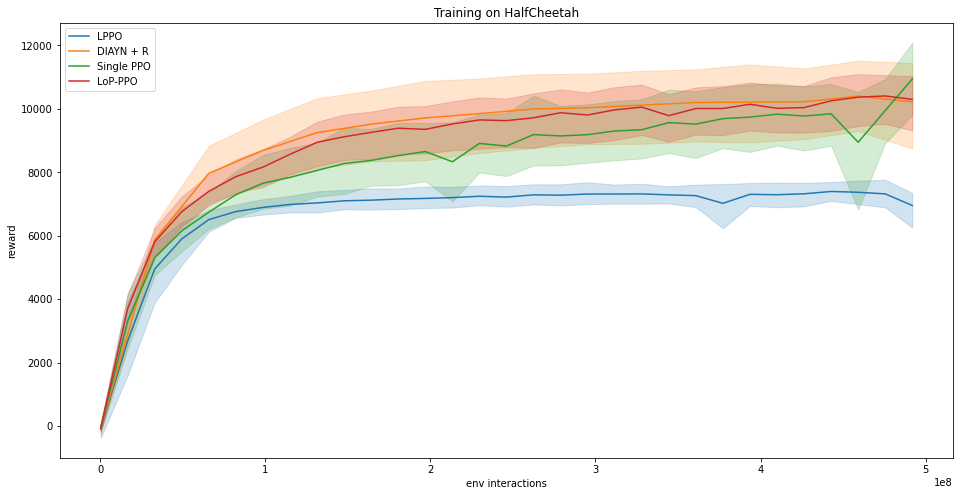
\includegraphics[width=1.0\textwidth]{images/halfcheetah_train.p%ng}
%\caption{Cumulative reward over training environment on HalfCheetah. %Results are averaged on 10 runs. For DIAYN + reward, we report the %results for $K=10$ (the best models). \label{fig:halfcheetah_train}}
%\end{figure}
\begin{table}[h!]
\centering
version https://git-lfs.github.com/spec/v1
oid sha256:6778dfb20d58a070901993174e09749c0eb9200a5e6c313b36260d7c89d029eb
size 2333
 
\scriptsize{}
\begin{tabular}{l|c|c|c|c|c|c}
 &\textbf{Single Policy} &\textbf{LoP} &\textbf{DIAYN + R} &\textbf{Lc} &\textbf{BoP} &\textbf{CoP} \\ 
 & (\textbf{K=1}) & & & & &\\ \midrule
 \textbf{K=10}& & & & & \\
BigFeet &7433 ± 1988 &\textbf{8903 ± 246} &8472 ± 535 &8340 ± 888 &8147 ± 835 &8553 ± 1033 \\
BigFriction &8579 ± 2224 &\textbf{11982 ± 330} &10781 ± 1870 &10705 ± 2092 &9093 ± 2436 &10850 ± 1526 \\
BigGravity &7508 ± 2086 &\textbf{10578 ± 648} &9766 ± 1424 &9488 ± 1616 &8026 ± 1809 &9568 ± 803 \\
BigShins &7274 ± 898 &\textbf{8854 ± 153} &8276 ± 607 &8340 ± 986 &7831 ± 978 &8753 ± 866 \\
BigThig &7963 ± 1466 &\textbf{10335 ± 1001} &9644 ± 1323 &9427 ± 1532 &8080 ± 1676 &9591 ± 884 \\
BigTorso &7091 ± 2221 &\textbf{10023 ± 427} &9295 ± 1106 &9271 ± 1317 &7928 ± 1772 &9131 ± 928 \\
SmallFeet &5973 ± 2490 &8805 ± 495 &8255 ± 504 &8186 ± 1458 &6660 ± 1842 &\textbf{9210 ± 1063} \\
SmallFriction &8652 ± 1717 &\textbf{11434 ± 358} &10637 ± 1505 &10204 ± 1663 &8708 ± 2007 &10459 ± 1387 \\
SmallGravity &9004 ± 1665 &\textbf{11969 ± 341} &10568 ± 1906 &10444 ± 1984 &9569 ± 2418 &11334 ± 1429 \\
SmallShin &7492 ± 2999 &\textbf{10764 ± 147} &9990 ± 1107 &9933 ± 1315 &8441 ± 1801 &9898 ± 982 \\
SmallThig &8914 ± 1837 &\textbf{11524 ± 298} &10689 ± 1137 &10632 ± 1170 &9430 ± 1881 &10600 ± 1473 \\
SmallTorso &8885 ± 1522 &\textbf{11567 ± 381} &10328 ± 1736 &10273 ± 1917 &9228 ± 1736 &10541 ± 1135 \\
HugeFriction &6999 ± 3441 &\textbf{11659 ± 307} &10335 ± 1955 &10379 ± 2302 &8526 ± 2710 &10899 ± 1541 \\
HugeGravity &6133 ± 2147 &\textbf{8793 ± 791} &8124 ± 1086 &7811 ± 1115 &6573 ± 1138 &8071 ± 352 \\
TinyFriction &7953 ± 1843 &\textbf{10662 ± 385} &10003 ± 1226 &9661 ± 1497 &7840 ± 2019 &9523 ± 1537 \\
TinyGravity &7304 ± 3484 &\textbf{11578 ± 460} &9723 ± 2167 &9650 ± 2228 &9221 ± 2224 &5107 ± 6910 \\\bottomrule
\textbf{Average} &7697 &\textbf{10589} &9680 &9547 &8331 &9506 \\\bottomrule
\vspace{0.5cm}
\end{tabular}


version https://git-lfs.github.com/spec/v1
oid sha256:ee31dc9dabd9565e8562347a53332e5600995a17320786912aa51cb6ceac9e06
size 2030

\caption{Mean and standard deviation of cumulative reward achieved on HalfCheetah test sets per model (see Table \ref{table:halfcheetah_test_setting} for environment details). Results are averaged over 10 training seeds (i.e., 10 models are trained with the same hyper-parameters and evaluated on the 16 test environments). $K$ is the number of policies tested at adaptation time, using 1 episode per policy since this environment is deterministic. Ensembling with $K=5$ models takes $5$ times more iterations to converge and testing values of $K>5$ is very costly in terms of GPU consumption.}
\label{table:halfcheetah_test}
\end{table}

% \begin{figure}[h!]
% \center
%     \begin{subfigure}{0.8\textwidth}
%         \begin{center}
%         \includegraphics[width=1\textwidth]{images/halfcheetahverybigfriction.png}
%           \end{center}
%     \end{subfigure}
%     \begin{subfigure}{0.8\textwidth}
%             \begin{center}
%     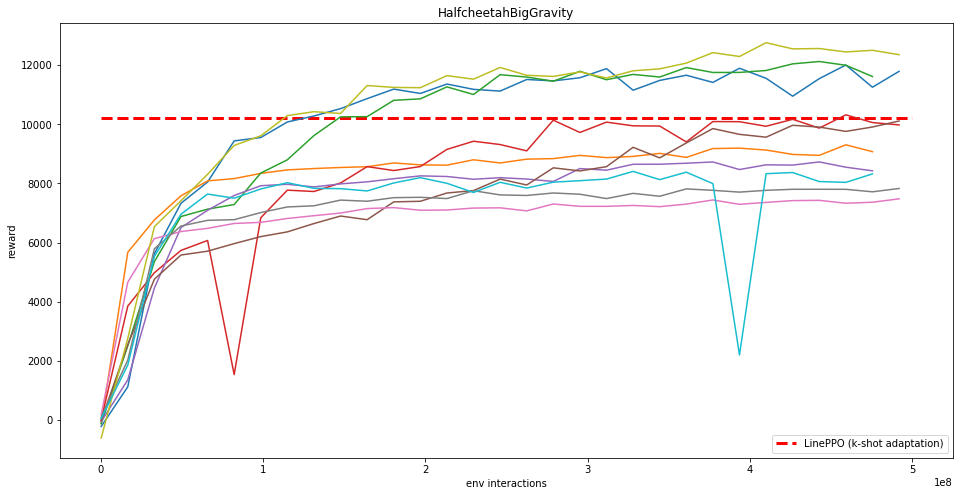
\includegraphics[width=1\textwidth]{images/halfcheetahbiggravity.png}
%       \end{center}
%     \end{subfigure}
%     \begin{subfigure}{0.8\textwidth}
%             \begin{center}
%     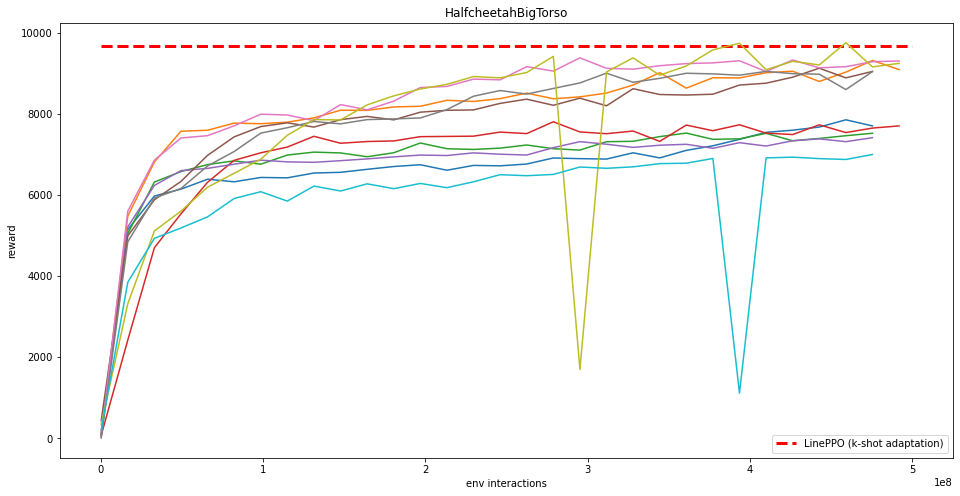
\includegraphics[width=1\textwidth]{images/halfcheetahbigtorso.png}
%     \end{center}
%     \end{subfigure}
% \caption{PPO models trained from scratch on test environments. For each environment, we launched 10 runs and compared the evolution of cumulative rewards to the performance of LoP in 100-shot adaptation (i.e. an exhaustive search on the line of parameters between the two anchor parameters). We use 100-shot to compare the sample-efficiency of LoP versus training from scratch: a 100-shots adaptation corresponds to $1e^5$ environment interactions. The curves show that the performance reached by LoP w.r.t a policy trained from scratch at test time is competitive in the three environments. results.).\label{fig:halfcheetah_from_scratch}}
% \end{figure}

\newpage

\begin{figure}[t]
        \begin{center}
        \includegraphics[width=1.\linewidth]{images/bigshin.png}
        \caption{Qualitative example of LoP trajectories on HalfCheetah "BigShins" test environment (5-shot setting). The best reward is obtained for $z=0.75$.}
        \label{fig:bigshin}
        \end{center}
\end{figure}

\vspace{5cm}

\begin{figure}[t]
        \begin{center}
        \includegraphics[width=1.\linewidth]{images/hugetorso.png}
        \caption{Extreme case: when torso radius and mass are increased by 50\%. Only one policy is able to adapt without falling down ($z=0.5$).}
        \label{fig:hugetorso}
        \end{center}
\end{figure}


.

\newpage

\begin{figure}[h!]
\centering
\includegraphics[width=0.55\linewidth]{images/hist_k5_halfcheetah_bis.png} \\
\includegraphics[width=0.55\linewidth]{images/hist_k10_halfcheetah.png} \\
\includegraphics[width=0.55\linewidth]{images/hist_k20_halfcheetah.png}
\caption{Number of times (y-axis) each policy (x-axis) is chosen by k-shot evaluation over the 16 test environments of the HalfCheetah for each of the 10 seeds (one table per seed). In \textcolor{blue}{blue}, LoP, in \textcolor{orange}{orange}, DIAYN+R. Please note that the 10 same LoP models are used for K=5, K=10, K=20 which is not the case for DIAYN+R.}
\label{fig:histograms}
\end{figure}

\newpage
.
\vspace{3.5cm}

\begin{figure}[h!]
\centering
\includegraphics[width=1.\linewidth]{images/discriminator_accuracy.png}
\caption{We trained small discriminators over a dataset (100,000 environment interactions) of trajectories obtained with the learned policies of LoP and DIAYN+R when K=5. For each environment, for each seed, we trained a single discriminator and averaged the results. While the discriminators trained on DIAYN+R reach 100\% accuracy rapidly on both train and test environments, they learn slower for LoP, with a slight advantage for the test environment, validating the fact that the diversity induced by the cosine similarity on the weights is more visible in variations of the environment rather than the environment on which the model has been trained. We evaluated the discriminator on a validation dataset (also 100,000 environment interactions) resulting in 100\% accuracy for DIAYN in both train and test environments. For LoP, we obtained 82\% accuracy on the training environment, and 87\% on the test environments. The discriminator architecture consists in a neural network of two hidden layers of size 16, taking the unprocessed states as an input and outputting the predicted policy used (like in DIAYN).}
\label{fig:discriminator_accuracy}
\end{figure}

\newpage
.
\vspace{3.5cm}

\begin{figure}[h!]
\centering
\includegraphics[width=1.\linewidth]{images/K_evolution.png}
\caption{Evolution of the best reward obtained with respect to K for LoP (N=2) and CoP (N=3) for each Halfcheetah test environment. We ran the K-shot evaluation for each K from K=1 to K=100 using the method described in Appendix \ref{subsec:bopcop}: we simply sample K random coefficients using the uniform distribution over $[0,1]$ for LoP and the Dirichlet distribution over $[0,1]^3$ for CoP. Results are averaged over 10 run for each K, and over the 10 models we learned for each method.  }
\label{fig:K_evolution}
\end{figure}

\newpage


\subsection{Ant}
\label{subsec:ant}

Task originally coming from OpenAI Gym (\cite{OpenaiGym}). Instead of using MuJoCo engine, we decided to use Brax (\cite{brax2021github}) as it enables the possibility to acquire episodes on GPU. We use the vanilla environment for training. The policy and the critic are encoded by two different multi-layer perceptrons with ReLU activations. The base learning algorithm is PPO.

\textbf{Test environments:}  As for HalfCheetah, we operated variations in physics (gravity and friction coefficients). We also designed environments with a percentage of masked features to simulate defective sensors (They are sampled randomly and remain the same for each run). Table \ref{table:ant_test_setting} precisely indicates the nature of the changes for each environment

\begin{table}[h!]
\centering
version https://git-lfs.github.com/spec/v1
oid sha256:05f8286e2b1298966c56902353a3a6be5fab5d8c6a7b5b64654b93fc246f2fd3
size 908

\label{table:ant_test_setting}
\end{table}

\newpage

\begin{table}[h!]
\begin{center}
\begin{tabular}{l|c} \toprule
   \textbf{Hyper-parameter} & \textbf{Value} \\ \hline
    lr policy: &  $0.0003$\\
    lr critic: &  $0.0003$\\
    n parallel environments: & $2048$ \\
    n acquisition steps per epoch: & $20$ \\
    batch size: & $1024$ \\
    num minibatches: & $16$ \\
    update epochs: & $16$ \\
    discount factor: &  $0.99$\\
    clip ration: &  $0.3$\\
    action std: &  $0.4$\\
    gae coefficient: &  $0.96$\\
    reward scaling: &  $1.$\\
    gradient clipping: & $10.$ \\ 
    n layers (policy): & $4$ \\ 
    n neurons per layer (policy): & $64$ \\
    n layers (critic): & $5$ \\ 
    n neurons per layer (critic): & $256$ \\
 \toprule
    \multicolumn{2}{c}{LoP} \\ 
    \hline
    $\beta$: & $\left \{ 0.1,1,10 \right \}$ \\
    \toprule
    \multicolumn{2}{c}{DIAYN} \\ 
    \hline
    $\beta$: & $\left \{ 0.1,1,10 \right \}$\\
    lr discriminator: &  $0.001$\\
    n layers (discriminator): & $2$ \\ 
    n neurons per layer (discriminator): &  $64$\\\hline
    \multicolumn{2}{c}{Lc} \\ 
    \hline
    $\beta$: & $\left \{ 0.1,1,10 \right \}$ \\
    dimensions of z: &  $1$\\
    lr discriminator: &  $0.001$\\
    n layers (discriminator): & $2$ \\ 
    n neurons per layer (discriminator): &  $64$\\\hline
\end{tabular}
\end{center}
\caption{Hyper-parameters for PPO over Ant}
\label{table:hp_ant}
\end{table}

\newpage

\begin{table}[h!]
\begin{adjustbox}{width=1.3\columnwidth,center}
\scriptsize{}
\begin{tabular}{l|c|ccc|ccc|ccc}
 &\multicolumn{1}{c}{\textbf{Single Policy}} &\multicolumn{3}{c}{\textbf{LoP}} & \multicolumn{3}{c}{\textbf{DIAYN + R}} &\multicolumn{3}{c}{\textbf{Lc}} \\ 
\multicolumn{1}{r|}{$\beta=$} & (K=1) & 0.1 & 1 & 10 & 0.1 & 1 & 10 & 0.1 & 1 & 10 \\
\midrule
\textbf{K=5} & & & & & & & & & & \\
BigFriction &7454 ± 166 &7544 ± 140 &7470 ± 96 &7541 ± 202 &7256 ± 1010 &6403 ± 726 &6267 ± 627 &\textbf{7666 ± 103} &7573 ± 154 &7538 ± 136 \\
BigGravity &6905 ± 138 &7038 ± 211 &6937 ± 23 &7027 ± 182 &6858 ± 827 &6082 ± 583 &5865 ± 543 &\textbf{7123 ± 184} &7075 ± 168 &7051 ± 131 \\
SmallFriction &6755 ± 2073 &7695 ± 156 &7652 ± 126 &7599 ± 167 &7046 ± 1777 &6491 ± 807 &6133 ± 706 &\textbf{7846 ± 127} &7673 ± 183 &7734 ± 211 \\
SmallGravity &7057 ± 1875 &7738 ± 134 &7639 ± 120 &7748 ± 169 &7533 ± 896 &6582 ± 727 &6486 ± 769 &\textbf{7876 ± 100} &7745 ± 105 &7772 ± 84 \\
HugeFriction &7505 ± 252 &7634 ± 152 &7616 ± 68 &7601 ± 253 &7220 ± 1331 &6387 ± 752 &6384 ± 733 &\textbf{7799 ± 103} &7647 ± 128 &7668 ± 77 \\
HugeGravity &380 ± 507 &1111 ± 538 &1407 ± 557 &1494 ± 934 &846 ± 556 &\textbf{2924 ± 1992} &2847 ± 1598 &1134 ± 934 &915 ± 465 &1440 ± 985 \\
TinyFriction &2747 ± 1241 &3716 ± 996 &\textbf{4584 ± 801} &4070 ± 1751 &3540 ± 948 &2950 ± 1113 &2600 ± 572 &3550 ± 843 &4140 ± 294 &3487 ± 508 \\
TinyGravity &-520 ± 426 &-106 ± 125 &-139 ± 274 &116 ± 322 &-479 ± 374 &-3 ± 202 &\textbf{224 ± 108} &-234 ± 790 &-401 ± 373 &-83 ± 329 \\
DefectiveSensor 5\% &4308 ± 59 &5243 ± 322 &\textbf{5630 ± 124} &5560 ± 272 &4958 ± 126 &4492 ± 211 &4360 ± 338 &5428 ± 424 &4988 ± 123 &5225 ± 562 \\
DefectiveSensor 10\% &2770 ± 171 &3620 ± 238 &\textbf{3660 ± 328} &3625 ± 291 &3440 ± 64 &3371 ± 57 &3223 ± 400 &3519 ± 76 &3406 ± 215 &3491 ± 207 \\
DefectiveSensor 15\% &1531 ± 90 &2583 ± 247 &2738 ± 312 &\textbf{2740 ± 167} &1774 ± 84 &1984 ± 383 &2055 ± 311 &2408 ± 340 &2226 ± 78 &2349 ± 271 \\
DefectiveSensor 20\% &1026 ± 77 &1750 ± 249 &1965 ± 234 &\textbf{2008 ± 199} &1104 ± 101 &1490 ± 387 &1450 ± 347 &1658 ± 245 &1546 ± 108 &1714 ± 238 \\
DefectiveSensor 25\% &736 ± 95 &1595 ± 317 &\textbf{1757 ± 154} &1526 ± 338 &762 ± 34 &1107 ± 396 &1120 ± 241 &1344 ± 262 &1271 ± 205 &1363 ± 254 \\
DefectiveSensor 30\% &472 ± 50 &695 ± 112 &793 ± 166 &674 ± 120 &577 ± 34 &\textbf{859 ± 290} &766 ± 212 &673 ± 115 &575 ± 49 &622 ± 100 \\
DefectiveSensor 35\% &424 ± 48 &606 ± 135 &\textbf{684 ± 182} &635 ± 85 &449 ± 68 &650 ± 245 &565 ± 151 &618 ± 170 &525 ± 92 &602 ± 175 \\
\bottomrule
\textbf{Average} &3338 &3905 &\textbf{4035} &3998 &3558 &3451 &3356 &3909 &3820 &3870 \\
\bottomrule
\end{tabular} 
\end{adjustbox}\\
\begin{adjustbox}{width=1.3\columnwidth,center}
version https://git-lfs.github.com/spec/v1
oid sha256:4df86496ab6ca43a493e5dcbbc7e6a5ca92b169ec9c00a6281a88b167d4f13eb
size 2542

\end{adjustbox}\\
\begin{adjustbox}{width=1.3\columnwidth,center}
version https://git-lfs.github.com/spec/v1
oid sha256:0caf23dd2cc007e642bd923fcf6645c96a4292231097223b785575a7085506a7
size 2541

\end{adjustbox}\\
\caption{Mean and standard deviation of cumulative reward achieved on Ant test sets per model. Results are averaged over 10 training seeds (i.e., 10 models are trained with the same hyper-parameters and evaluated on the 12 test sets). $K$ is the number of policies tested at adaptation time, using 1 episode per policy since this environment is deterministic. For this environment, we split the results per $\beta$ value as it has been used for beta ablation study (see Figure \ref{tab:beta_ablation})}
\end{table}
\label{table:ant_test_results}

\newpage

.
\vspace{4cm}

\begin{figure}[h!]
    \centering
    \includegraphics[width=1.\linewidth]{images/ant_beta.png}
    \caption{Evolution of the cumulative reward during training on the generic Ant environment for LoP, DIAYN+R and Lc for different values of beta. On can see that DIAYN+R struggles to perform well on the train set for $\beta=1$ and $\beta=10$. Results are averaged over 10 seeds.}
    \label{fig:ant_beta_train}
\end{figure}

\newpage

\subsection{CartPole}
\label{subsec:cartpole}

We use the openAI gym implementation of CartPole as a training environment. The 6 test environments are provided by \cite{PackerGao:1810.12282} where three different factors may vary: the mass of the cart, the length of the pole and the force applied to the cart. The length of each episode is 200.  The policy and the critic are encoded by two different multi-layer perceptrons with ReLU activations. The base learning algorithm is A2C.

\begin{table}[h!]
\begin{center}
\begin{tabular}{l|c} \toprule
\textbf{Environment} & \textbf{Characteristics} \\ \hline
(Train) CartPole & $mass=0.1, length=0.5 ,force=10.0$ \\ \hline
HeavyPole CartPole & $mass=1.0$ \\
LightPole CartPole &  $mass=0.001$ \\
LongPole CartPole & $length=1.0$ \\
ShortPole CartPole & $length=0.05$ \\
StrongPush CartPole & $force=20.0$ \\
WeakPush CartPole &  $force=1.0$\\
\hline
\end{tabular}
\end{center}
\caption{CartPole train and test environments}
\end{table}


\begin{table}[h!]
\begin{center}
\begin{tabular}{l|c} \toprule
   \textbf{Hyper-parameter} & \textbf{Value} \\ \hline
    learning rate: &  $0.001$\\
    n acquisition steps per epoch: & $8$ \\
    n parallel environments: &  $32$\\
    critic coefficient: &  $1.0$\\
    entropy coefficient: &  $0.001$\\
    discount factor: &  $0.99$\\
    gae coefficient: &  $1.0$\\
    gradient clipping: & $2.0$ \\ 
    n neurons per layer: & $8$ \\
    n layers: & $2$ \\
 \toprule
    \multicolumn{2}{c}{LoP} \\ 
    \hline
    $\beta$: & $1.0$ \\
    \toprule
    \multicolumn{2}{c}{DIAYN} \\ 
    \hline
    $\beta$: & $1.0$ \\
    n neurons per layer discriminator: & $8$ \\
    n layers discriminator: & $2$ \\
    learning rate discriminator: & $0.001$ \\ \hline
\end{tabular}
\end{center}
\caption{Hyper-parameters for A2C over CartPole}
\label{table:hp_cartpole}
\end{table}

\begin{table}[h!]
\begin{center}
    \begin{tabular}{l|c|c|c|c} \toprule
    &	Single	& LoP &	DIAYN+R& 	DIAYN+R $L_2$	\\ \hline
HeavyPole CartPole	&	200.0 ± 0.0	& 200.0 ± 0.0	& 200.0 ± 0.0	& 200.0 ± 0.0	\\ 
LightPole CartPole	&	200.0 ± 0.0	& 200.0 ± 0.0	& 200.0 ± 0.0	& 200.0 ± 0.0	\\ 
LongPole CartPole	&	54.4 ± 81.6	& 56.1 ± 72.2	& 163.3 ± 73.3	& 123.8 ± 86.2	\\ 
ShortPole CartPole	&	67.0 ± 33.1	& 78.9 ± 25.3	& 50.7 ± 18.1	& 64.8 ± 31.2	\\ 
StrongPush CartPole	&	200.0 ± 0.0	& 200.0 ± 0.0	& 200.0 ± 0.0	& 199.9 ± 0.2	\\ 
WeakPush CartPole	&	138.9 ± 43.8	& 164.4 ± 18.3	& 194.3 ± 10.0	& 148.1 ± 64.8	\\ \hline
Average	&	143.4	&149.9&	\textbf{168.1} &	156.1\\
\hline
\end{tabular}
\caption{Results over CartPole, using 10 policies, and 10 episodes per policy at adaptation time. }
\end{center}
\end{table}
\newpage

\subsection{AcroBot}
\label{subsec:acrobot}

We use the openAI gym implementation of Acrobot as a training environment. The 4 test environments are provided by \cite{PackerGao:1810.12282} where two different factor may vary: the intertia factor and the lengh of the system. We have used A2C as a learning algorithm.


\begin{table}[h!]
\begin{center}
\begin{tabular}{l|c} \toprule
\textbf{Environment} & \textbf{Characteristics} \\ \hline
(Train) Acrobot & $mass=0.1, length=1.0 ,inertia=1.0$ \\ \hline
Heavy Acrobot  & $mass=1.5$ \\
HighInertia Acrobot  &  $inertia=1.5$ \\
Light Acrobot  & $mass=0.5$\\
Long Acrobot  & $length=1.5$ \\
LowInertia Acrobot  & $inertia=0.5$ \\
Short Acrobot  &  $length=0.5$\\
\hline
\end{tabular}
\end{center}
\caption{Acrobot train and test environments}
\end{table}


\begin{table}[h!]
\begin{center}
\begin{tabular}{l|c} \toprule
   \textbf{Hyper-parameter} & \textbf{Value} \\ \hline
    learning rate: &  $0.001$\\
    n acquisition steps per epoch: & $8$ \\
    n parallel environments: &  $32$\\
    critic coefficient: &  $1.0$\\
    entropy coefficient: &  $0.001$\\
    discount factor: &  $0.99$\\
    gae coefficient: &  $0.7$\\
    gradient clipping: & $2.0$ \\ 
    n neurons per layer: & $16$ \\
    n layers: & $2$ \\ \toprule
    \multicolumn{2}{c}{LoP} \\  \hline
    $\beta$: & $1.0$ \\
    \toprule
    \multicolumn{2}{c}{DIAYN} \\ \hline
    $\beta$: & $1.0$ \\
    n neurons per layer discriminator: & $16$ \\
    n layers discriminator: & $2$ \\
    learning rate discriminator: & $0.001$ \\ \hline
\end{tabular}
\end{center}
\caption{Hyper-parameters for A2C over Acrobot}
\label{table:hp_acrobot}
\end{table}


\begin{table}[h!]
\begin{center}
    \begin{tabular}{l|c|c|c|c} \toprule
    &	Single	& LoP &	DIAYN+R& 	DIAYN+R $L_2$	\\ \hline
Heavy Acrobot	&	-108.4 ± 3.2	& -105.1 ± 1.0	& -108.0 ± 1.8	& -108.2 ± 4.4	\\
HighInertia Acrobot	&	-108.7 ± 5.6	& -99.8 ± 2.8	& -106.0 ± 2.7	& -106.8 ± 8.9	\\
Light Acrobot	&	-120.7 ± 71.3	& -107.2 ± 58.8	& -115.2 ± 33.1	& -93.1 ± 37.3	\\
Long Acrobot	&	-124.3 ± 2.7	& -115.8 ± 9.6	& -117.3 ± 4.1	& -117.5 ± 5.3	\\
LowInertia Acrobot	&	-71.3 ± 2.3	& -70.7 ± 0.7	& -71.2 ± 0.7	& -71.3 ± 1.9	\\
Short Acrobot	&	-65.1 ± 2.8	& -60.7 ± 0.6	& -64.2 ± 2.6	& -64.7 ± 5.6	\\ \hline
Average	&	-99.7&	\textbf{-93.2} &	-97.0&	-93.6\\
\hline
\end{tabular}
\caption{Results over Acrobot, using 10 policies, and 10 episodes per policy at adaptation time. }
\end{center}
\end{table}
\newpage
\subsection{Pendulum}
\label{subsec:pendulum}

We use the openAI gym implementation of Pendulum as a training environment. The 3 test environments are provided by \cite{PackerGao:1810.12282} where two different factor may vary: the mass and the length of the pendulum. We have considered 5 discrete actions between $-1$ and $+1$. We have used A2C as a learning algorithm.



\begin{table}[h!]
\begin{center}
\begin{tabular}{l|c} \toprule
\textbf{Environment} & \textbf{Characteristics} \\ \hline
(Train) Pendulum & $mass=1.0, length=1.0$ \\ \hline
Light Pendulum  & $mass=0.5$ \\
Long Pendulum &  $length=1.5$ \\
Short Pendulum  & $length=0.5$ \\
\hline
\end{tabular}
\end{center}
\caption{Pendulum train and test environments}
\end{table}


\begin{table}[h!]
\begin{center}
\begin{tabular}{l|c} \toprule
   \textbf{Hyper-parameter} & \textbf{Value} \\ \hline
    learning rate: &  $0.001$\\
    n acquisition steps per epoch: & $8$ \\
    n parallel environments: &  $32$\\
    critic coefficient: &  $1.0$\\
    entropy coefficient: &  $0.001$\\
    discount factor: &  $0.99$\\
    gae coefficient: &  $0.7$\\
    gradient clipping: & $2.0$ \\ 
    n neurons per layer: & $16$ \\
    n layers: & $2$ \\ \toprule
    \multicolumn{2}{c}{LoP} \\  \hline
    $\beta$: & $1.0$ \\
    \toprule
    \multicolumn{2}{c}{DIAYN} \\ \hline
    $\beta$: & $1.0$ \\
    n neurons per layer discriminator: & $16$ \\
    n layers discriminator: & $2$ \\
    learning rate discriminator: & $0.001$ \\ \hline
\end{tabular}
\end{center}
\caption{Hyper-parameters for A2C over Pendulum}
\label{table:hp_pendulum}
\end{table}


\begin{table}[h!]
\begin{center}
    \begin{tabular}{l|c|c|c|c} \toprule
    &	Single	& LoP &	DIAYN+R& 	DIAYN+R $L_2$	\\ \hline
    
    Light Pendulum	&	-36.5 ± 58.5	& -11.4 ± 2.7	& -39.3 ± 10.9	& -32.1 ± 15.4	\\
Long Pendulum	&	-82.1 ± 20.4	& -64.5 ± 13.0	& -70.6 ± 15.2	& -71.9 ± 17.3	\\
Short Pendulum	&	-39.6 ± 66.9	& -10.7 ± 2.1	& -31.3 ± 11.7	& -28.2 ± 13.3	\\ \hline
Average	&	-52.7	& \textbf{-28.9}	& -47.1	& -44.0	\\
\hline
\end{tabular}
\caption{Results over Pendulum, using 10 policies, and 10 episodes per policy at adaptation time. }
\end{center}
\end{table}
\newpage
\subsection{MiniGrid}
\label{subsec:minigrid}

We have use Gym Minigrid to perform experiments on mazes \cite{gym_minigrid}. We have used the MultiRoom-N2-S4 for training considering one single maze. At test time, we have tested on three different MultiRoom-N2-S4 environments  composed of two rooms, but also on three MultiRoom-N4-S5  composed of four rooms. This allows us to evaluate the generalization power of the different methods to larger mazes. We have used A2C as a learning algorithm.


\begin{table}[h!]
\begin{center}
\begin{tabular}{l|c} \toprule
   \textbf{Hyper-parameter} & \textbf{Value} \\ \hline
    learning rate: &  $0.001$\\
    n acquisition steps per epoch: & $8$ \\
    n parallel environments: &  $32$\\
    critic coefficient: &  $1.0$\\
    entropy coefficient: &  $0.001$\\
    discount factor: &  $0.99$\\
    gae coefficient: &  $0.7$\\
    gradient clipping: & $2.0$ \\ 
    n neurons per layer: & $16$ \\
    n layers: & $2$ \\ \toprule
    \multicolumn{2}{c}{LoP} \\ \hline
    $\beta$: & $1.0$ \\ \toprule
    \multicolumn{2}{c}{DIAYN} \\ \hline
    $\beta$: & $1.0$ \\
    n neurons per layer discriminator: & $16$ \\
    n layers discriminator: & $2$ \\
    learning rate discriminator: & $0.001$ \\ \hline
\end{tabular}
\end{center}
\caption{Hyper-parameters for A2C over Minigrid}
\label{table:hp_minigrid}
\end{table}


\begin{table}[h!]
\begin{center}
    \begin{tabular}{l|c|c|c|c} \toprule
        &	Single	& LoP &	DIAYN+R& 	DIAYN+R $L_2$	\\ \hline

Two Rooms Maze 1	&	0.387 ± 0.447	& 0.619 ± 0.309	& 0.348 ± 0.348	& 0.656 ± 0.328	\\ 
Two Rooms Maze 2	&	0.433 ± 0.499	& 0.865 ± 0.0	& 0.627 ± 0.363	& 0.692 ± 0.346	\\ 
Two Rooms Maze 3	&	0.194 ± 0.387	& 0.617 ± 0.309	& 0.348 ± 0.353	& 0.656 ± 0.328	\\ 
Four Rooms Maze 1	&	0.0 ± 0.0	& 0.294 ± 0.36	& 0.0 ± 0.0	& 0.24 ± 0.359	\\ 
Four Rooms Maze 2	&	0.0 ± 0.0	& 0.004 ± 0.007	& 0.0 ± 0.0	& 0.137 ± 0.274	\\ 
Four Rooms Maze 3	&	0.0 ± 0.0	& 0.281 ± 0.345	& 0.166 ± 0.287	& 0.28 ± 0.345	\\ \hline
Average	&	0.169	& \textbf{0.447}	& 0.248	& 0.443	\\
\hline
\end{tabular}
\caption{Results over Minigrid, using 10 policies, and 1 episode per policy at adaptation time. }
\end{center}
\end{table}

\newpage
\subsection{ProcGen (FruitBot)}
\label{subsec:procgen}

We performed experiments on pixel-based environment with ProcGen. We used the FruitBot game for training considering 10 levels sampled uniformly at each episode. At test time, we selected 3 different environments, each of them composed of 10 uniformly sampled levels, sampled uniformly, and that were not seen at train time. We used the CNN architecture described in the ProcGen paper (IMPALA architecture (\cite{espeholt2018impala})). For LoP, the two first blocks are fixed and only the parameters of the last block depend on the value of $z$. For DIAYN, the $z$ value is provided as a one-hot vector stacked to the observation. As for Brax environment, we used PPO algorithm.




\begin{table}[h!]
\begin{center}
\begin{tabular}{l|c} \toprule
   \textbf{Hyper-parameter} & \textbf{Value} \\ \hline
    learning rate: &  $5e-4$\\
    n acquisition steps per rollout: & $128$ \\
    n batches epoch: & $8$ \\
    n epochs per rollout: & $5$ \\
    n parallel environments: &  $64$\\
    critic coefficient: &  $1.0$\\
    entropy coefficient: &  $0.01$\\
    discount factor: &  $0.99$\\
    gae coefficient: &  $0.0$\\
    gradient clipping: & $20.0$ \\ 
    \multicolumn{2}{c}{LoP} \\ \hline
    $\beta$: & $0.01,0.1,1.0$ \\ \toprule
    \multicolumn{2}{c}{DIAYN+R} \\ \hline
    $\beta$: & $0.001,0.01,0.1,1.0$ \\ \hline
\end{tabular}
\end{center}
\caption{Hyper-parameters for PPO over ProcGen}
\label{table:hp_procgen}
\end{table}


\begin{table}[h!]
\begin{center}
    \begin{tabular}{l|c|c|c|} \toprule
        &	Single	& LoP &	DIAYN+R 	\\ \hline

Levels 100 to 110	&	11.9 ± 2.6	& 20.1 ± 4.4	& 12.1 ± 5.2		\\ 
Levels 200 to 210	&	7.1 ± 1.7	& 10.3 ± 0.2	& 5.1 ± 1.7		\\ 
Levels 300 to 310	&	14.3 ± 5.1	& 18.7 ± 2.7	& 17.1 ± 4.6		\\ \hline
\end{tabular}
\caption{Results over Procgen, using K=10 at adaptation time, (averaged over 16 episodes per shot), averaged over 5 runs. }
\end{center}
\end{table}


\newpage

\subsection{Maze 2d with walls}
\label{subsec:maze2d}

To visualize the policies learned by the different methods, we just implemented a simple discrete maze (4 actions = up,down, left, right) where the objective is to go from the top-middle tile to the bottom-middle tile by moving through a corridor (size is $21 \times 11$). Reward is -1 at each step until goal is reached and the maximum number of steps is $-100$. The optimal policy in the training environment achieves $-16$.  At test time, we generate walls in the corridor such that the agent has to avoid these walls to reach the goal. The observation space is a $5 \times 5$ square around the agent. Policies are learned by using PPO. 
Illustrations of the trajectories over the train and the 4 test environments are illustrated in Figures \ref{fig:maze1},\ref{fig:maze2},\ref{fig:maze3},\ref{fig:maze4}

\begin{table}[h!]
\begin{center}
\begin{tabular}{l|c} \toprule
   \textbf{Hyper-parameter} & \textbf{Value} \\ \hline
    learning rate: &  $0.001$\\
    n acquisition steps per rollout: & $16$ \\
    n batches epoch: & $4$ \\
    n epochs per rollout: & $3$ \\
    n parallel environments: &  $32$\\
    critic coefficient: &  $1.0$\\
    entropy coefficient: &  $0.01$\\
    discount factor: &  $0.99$\\
    gae coefficient: &  $0.0$\\
    gradient clipping: & $20.0$ \\ 
    \multicolumn{2}{c}{LoP} \\ \hline
    $\beta$: & $0.01,0.1,1.0$ \\ \toprule
    \multicolumn{2}{c}{DIAYN+R} \\ \hline
    $\beta$: & $0.01,0.1,1.0$ \\ \hline
\end{tabular}
\end{center}
\caption{Hyper-parameters for PPO used for Maze 2d}
\label{table:hp_maze}
\end{table}

\begin{table}[h!]
\centering
\scriptsize{}
\begin{tabular}{l|c|ccc|ccc}
& \textbf{Single Policy} & \multicolumn{3}{c}{\textbf{LoP}} & \multicolumn{3}{c}{\textbf{DIAYN + R}} \\ 
\multicolumn{1}{r|}{$\beta=$}  &  & 0.01 & 0.1 & 1. & 0.01 & 0.1 & 1. \\
\midrule
Test Env \#1  & -16.0 ± 0.0 &-17.6 ± 2.2 &-17.2 ± 1.1 &-17.6 ± 2.6 &\textbf{-16 ± 0} &-16 ± 0 &-16 ± 0 \\
Test Env \#2  & -100 ± 0.0 &\textbf{-23.6 ± 3.6} &-39.4 ± 25.8 &-30.2 ± 11.6 &-56.2 ± 40.2 &-42.6 ± 33 &-44.8 ± 31.5 \\
Test Env \#3 & -100 ± 0.0 &\textbf{-37.8 ± 18.9} &-41.6 ± 10.6 &-43.6 ± 11.5 &-54.2 ± 27.1 &-55.8 ± 31.4 &-60.4 ± 27 \\
Test Env \#4  & -100 ± 0.0 &\textbf{-42.2 ± 11.8} &-60.8 ± 27.9 &-48 ± 22.9 &-54.8 ± 28.9 &-53.4 ± 26.5 &-72.8 ± 33.8 \\
Test Env \#4  & -100 ± 0.0 &\textbf{-28.4 ± 10.7} &-44.4 ± 30.2 &-28.8 ± 8.9 &-37.4 ± 35.4 &-43.2 ± 34.7 &-50.4 ± 38.8 \\
\bottomrule
\textbf{Average} & -83.2 & \textbf{-29.9} &-40.68 &-33.64 &-43.72 &-42.2 &-48.88 \\
\bottomrule
\end{tabular}
\caption{Results over Maze2d, using K=10, averaged over 5 runs. }
\label{table:maze2d_results}
\end{table}

\begin{figure}[h!]
    \centering
    \includegraphics[width=0.5\linewidth]{images/SINGLEPOLICY.png}
    \caption{Trajectories learned by a Single Policy. First column is the training environment. Other columns are test environments. The lighter red the tiles are, the longer the agent stays on a particular location.}
    \label{fig:maze1}
\end{figure}

\begin{figure}[h!]
    \centering
    \includegraphics[width=0.75\linewidth]{images/LOP1.png}
    \caption{Trajectories learned by LoP ($\beta=1.0$). Rows are environments, columns are the $K=10$ policies test during online adaptation. For each test environment, at least one policy is able to reach the goal}
    \label{fig:maze2}
\end{figure}

\begin{figure}[h!]
    \centering
    \includegraphics[width=0.75\linewidth]{images/DIAYN0.01.png}
    \caption{Trajectories learned by DIAYN+R ($\beta=0.01$). Rows are environments, columns are the $K=10$ policies test during online adaptation. For many test environment, at least one policy is able to reach the goal}
    \label{fig:maze3}
\end{figure}

\begin{figure}[h!]
    \centering
    \includegraphics[width=0.75\linewidth]{images/DIAYN1.png}
    \caption{Trajectories learned by DIAYN+R ($\beta=1$).  Rows are environments, columns are the $K=10$ policies test during online adaptation. With a too high value of $\beta$, the training policy is suboptimal, and does not achieve good performance at train and test times.}
    \label{fig:maze4}
\end{figure}